\documentclass{article}
\usepackage{tikz}
\usepackage{amsmath}

\begin{document}

\begin{center}
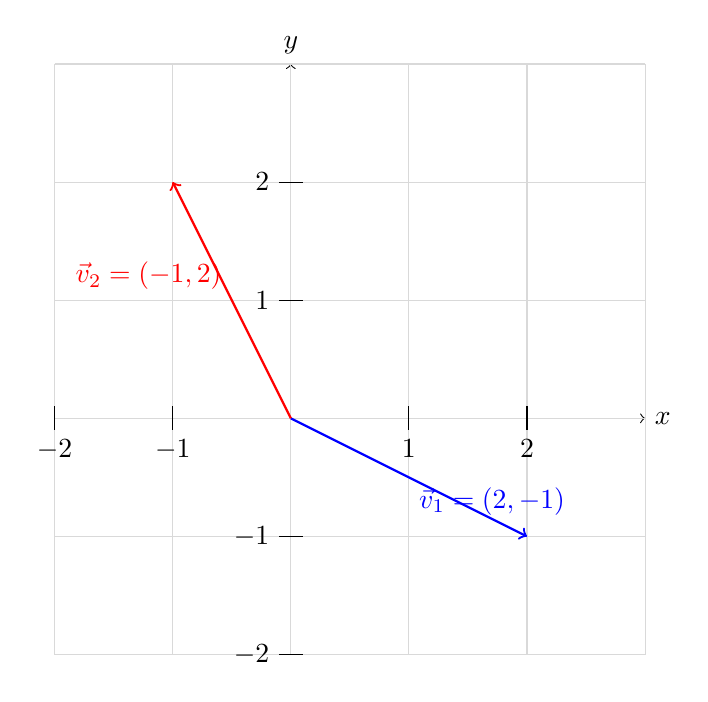
\begin{tikzpicture}[scale=1.5]
    % Draw coordinate axes
    \draw[->] (-2,0) -- (3,0) node[right] {$x$};
    \draw[->] (0,-2) -- (0,3) node[above] {$y$};
    
    % Draw grid
    \draw[gray!30] (-2,-2) grid (3,3);
    
    % Draw vectors
    \draw[->, thick, blue] (0,0) -- (2,-1) node[midway, below right] {$\vec{v}_1 = (2,-1)$};
    \draw[->, thick, red] (0,0) -- (-1,2) node[midway, above left] {$\vec{v}_2 = (-1,2)$};
    
    % Add some points for reference
    \foreach \x in {-2,-1,1,2}
        \draw (\x,0.1) -- (\x,-0.1) node[below] {$\x$};
    \foreach \y in {-2,-1,1,2}
        \draw (0.1,\y) -- (-0.1,\y) node[left] {$\y$};
\end{tikzpicture}
\end{center}

\end{document} 